\documentclass[11pt,twocolumn]{article}
\usepackage[margin=1.0in]{geometry}
\usepackage{blindtext}
\usepackage[utf8]{inputenc}
\usepackage{listings}
\usepackage{graphicx} %package to manage images
%\usepackage{multicol}
\usepackage{xcolor}
\usepackage{csquotes}
\usepackage{paralist}
\setlength{\columnsep}{25pt}
\graphicspath{ {images/} }

\title{BPMN to PROMELA}
\author{Jamie Visker}
\date{\today}
 
\begin{document}

\maketitle
% \begin{multicols}{2}

\lstset{
    basicstyle=\footnotesize,
    numbers=left,
    frame=single,
    breaklines=true,
    postbreak=\raisebox{0ex}[0ex][0ex]{\ensuremath{\color{red}\hookrightarrow\space}}
}

\begin{abstract}
BPMN is a visual process modelling language. It is helpful in formalizing business processes, but can easily have unintended behavior. This work presents a novel translation process that converts the BPMN language into PROMELA, a language consumable by the model checker SPIN. Then SPIN can check for valid end states, data-race freedom, and user defined property validity.

BPMN execution is represented with a \emph{token} that moves along interconnecting arrows and objects. Our translation represents the location of tokens with counters. Movement in the system is modelled with a switch like structure. The switch statement is repeated until the token reaches the end of a process.

Objects in the diagram can be enabled by tokens entering after which they can execute. The translation creates PROMELA processes with the correct transitions. It also allows for communication between processes using message passing methods in PROMELA.

Our experiments were small but generated valid PROMELA. Future work will require that techniques are employed to help maintain the state space.
\end{abstract}

\begin{figure*}
 \begin{center}
  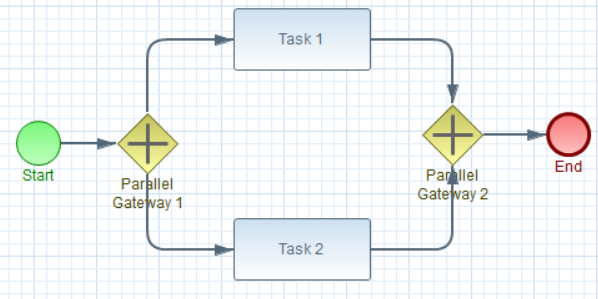
\includegraphics[width=100mm]{simpleFlow}
  \end{center}
  \caption{A Simple BPMN Flow}
  \label{fig:simpleFlow}
\end{figure*}

\section{Introduction}
BPMN is a visual language that allows for the expression of business processes. Using BPMN, business users can formalize their processes and improve their analysis of their models. Although BPMN is a visual language it is just as likely to have unintended behavior as say a C++ or Java program. For example, a BPMN model could easily introduce data race conditions, deadlocks, or terminating in an unexpected or invalid state. It is important that we can report to users when there is a problem, especially when the processes are critical to safety or health. For example, BPMN diagrams are not uncommon in specifying flows for hospitals and patient management. In these contexts, it is important that processes safeguard patient health and privacy. There are many different BPMN execution engines that will allow you to simulate BPMN models. These solutions try possibilities to understand the average case performance of the model but say nothing definitive about the correctness of the process or its ability to accomplish its intended work. 

In contrast, we propose a new method that uses model checking to formally verify the correctness of the BPMN models. Where simulation may consistently miss behaviors that lead to errors because it is random, model checking considers every possible behavior, no matter how improbable, to find errors. In addition to finding error we can also prove properties about things that should happen in a system. In this way we can report definitively the correctness of a process.

In taking on this challenge we have restricted the scope for our first attempt. There are several different branches of BPMN models such as \emph{Processes}, \emph{Collaborations}, \emph{Choregoraphies}, and \emph{Conversations}. Our focus is on \emph{Processes}, though the techniques we present may be applicable to the other types of models in the future. Beyond this we have had to restrict the types of BPMN Elements that can be used. These restrictions are not trivial and eliminate many classes of problems, such as those that model any type of loop. There are, however, many real world problems that can be modeled with the restrictions we have in place.

We are using the model checking tool \emph{SPIN} as our model checker. Therefore the work of this paper mainly deals with a translation between BPMN and PROMELA, the language of SPIN. The translation process involves two steps. First the BPMN model files must be parsed and imported into a program. Then that program can do the translation to PROMELA. We have not implemented the import, but rather have built an API that an importer may use. The experiments presented in this report manually exercise the interface to construct the data structure while future work would automate that process building the data-structure from the XML representation of the BPMN diagram. 

BPMN processes are converted into PROMELA processes. Our approach is to represent sequence flows with counters and use a PROMELA construct to represent a transition function within each process. This transition system allows us to compactly represent tokens moving through a BPMN diagram.

Our translation method was inspired by BPMN to Petri net conversion. Petri Nets have a formally defined semantics with several analysis tools that provide verification services. As a formalism, Petri Nets naturally express concurrency over events, but are much less intuitive to draw and typically do not include data directly. BPMN is intended to be more intuitive and approachable to business applications when compared to Petri Nets. In contrast to Petri nets, however, we add the concept of data and data flow which is not naturally compatible with Petri nets. Our translation captures the use of Data using BPMN's \emph{Data Store} and \emph{Data Object} and is discussed in Section \ref{sec:data}.

The rest of the paper is organized as follows: Section 2 provides a simple overview of the project; Section 3 provides background on BPMN and PROMELA Semantics; Section 4 gives translation techniques to transform BPMN to PROMELA; Section 5 discusses validation done on the translation; Section 6 discusses Related Work; Section 7 provides Conclusions and Future Work; and finally Section 8 lists other notes and assumptions about the translation.
\section{Example}

BPMN processes are intended to model business work-flows but can be used to describe any work-flow. Consider the BPMN process model in Figure \ref{fig:simpleFlow}. The circles represent \emph{events}. Events start or stop the process. The diamonds represent \emph{gateways}. Gateways implement control flow through the process. The rectangles are \emph{tasks}. Tasks represent where work takes place. The arrows connecting the different components are \emph{flows}. Flows connect events, gateways, and tasks. 

The BPMN process semantics can be understood with the schema of \emph{tokens} that flow through the diagram. A token is an abstract object that coordinates activation of the different elements of the process. Events produce and consume tokens. For the process in Figure \ref{fig:simpleFlow}, it is activated by placing a single token in the start-event. The start-event then places that token on its outgoing flow. The process ends when that same token arrives at the incoming flow to the end-event on the right. The end-event takes a single token on its incoming flow and consumes it. Events come in several varieties as discussed in Section \ref{sec:background}. 

In general, tokens on incoming flows \emph{enable} things. Enabled means that the thing connected to the flows is able to activate and then move the tokens to its outgoing flows according to its semantics. Those semantics may split the tokens into more tokens or merge many tokens into a single token.  

Consider the gateways in Figure \ref{fig:simpleFlow}. These are parallel gateways indicated by the \emph{plus} sign, so the gateway on the left, a parallel split, takes a token from its incoming flow and replicates it so that there is a token on each of its outgoing flows. The gateway on the right, a parallel join, takes a token from each of its incoming flows and merges them into a single token on its outgoing flow. Gateways come in two different varieties each with slightly different semantics as discussed in Section \ref{sec:background}. 

Tasks move tokens from their incoming flows to their outgoing flows. Moving a token across the task indicates that the task is completed. Tasks come in many varieties, including a notion of a task being decomposed into a sub-process. Most tasks can be configured to read data, write data, and have well defined delay bounds. It is also possible to indicate who or what accomplishes a task. These different things are discussed later in Section \ref{sec:background}. 

The goal of the project discussed in this paper is to verify three types of properties in any given BPMN process:
\begin{compactitem}
\item \emph{Valid end states}: all tokens are consumed by end-events
\item \emph{Data-race freedom}: all data accesses do not conflict
\item \emph{User defined properties}: all assertions and temporal logic statements are satisfied 
\end{compactitem}
Conflict in data-race means that there are concurrent accesses to a common data object and at least one access is a write. 

\begin{figure}[t]

\begin{lstlisting}
do
	:: ...
	::in_tokens(token_start) -> 
		atomic{
		print(997/*start*/);
		out_tokens(token_divParGW_1)
		}
	::in_tokens(token_end_6) -> 
		atomic{
		print(998/*end*/);
		break;
		}
	::in_tokens(token_task1_2) -> 
		atomic{
		print(996/*task1*/);
		
		x = 3;
		
		out_tokens(token_conParGW_4)
		}
	:: ...
od
\end{lstlisting}

\caption{A snippet of the PROMELA code from the translated process in Figure \ref{fig:simpleFlow}.}
\label{fig:promelaSmall}
\end{figure}

The goal is accomplished by automatically translating the BPMN process into the input language of the SPIN model checker and then verifying the resulting SPIN model for the indicated properties. A small snippet of the PROMELA model is shown in Figure \ref{fig:promelaSmall}. Without going into too much detail, the translation implements a \emph{switch-statement} in a looping structure using PROMELA's \emph{do-statement} (lines 1 -- 22). The do-statement enumerates cases (e.g., lines 3, 8, 13, etc.) over each of the objects of the process executing cases when they are valid.  A case tests if the object's incoming flow has sufficient tokens to be enabled, and if yes, it activates the object, accomplishes the work, and places tokens on the appropriate outgoing flows. The model checker exhaustively enumerates all schedules of activations in checking properties. 

\begin{figure}[t]
\begin{center}
\begin{lstlisting}
...
State-vector 36 byte, depth reached 27, errors: 0
       22 states, stored
        1 states, matched
       23 transitions (= stored+matched)
       13 atomic steps
hash conflicts:         0 (resolved)
...
unreached in proctype process_SimpleFlow
	generatedPromela.pml:37, state 59, "printf('token_conParGW_4 %d\n',token_conParGW_4)"
...
\end{lstlisting}
\end{center}
\caption{A snippet of the SPIN verification output for the translation of Figure \ref{fig:simpleFlow}.}
\label{fig:spinOutputSmall}
\end{figure}

For the example in Figure \ref{fig:simpleFlow}, the model checker only needs to check for valid end states since there are no data and no user properties. A snippet of the model checker output is shown in Figure \ref{fig:spinOutputSmall}. The input to the model checker is 62 lines of code in two processes. The output indicates that there are no errors (line 2), and it proved the absence of errors after exploring 22 states (line 3) and 23 transitions of the input model (line 4). The verification took .15 seconds. The verification report also includes portions of the input model that were not activated (line 9). This information is extremely helpful in developing the process model since it indicates \emph{dead-code} (e.g., parts of the process that never activate). 

\begin{figure*}
  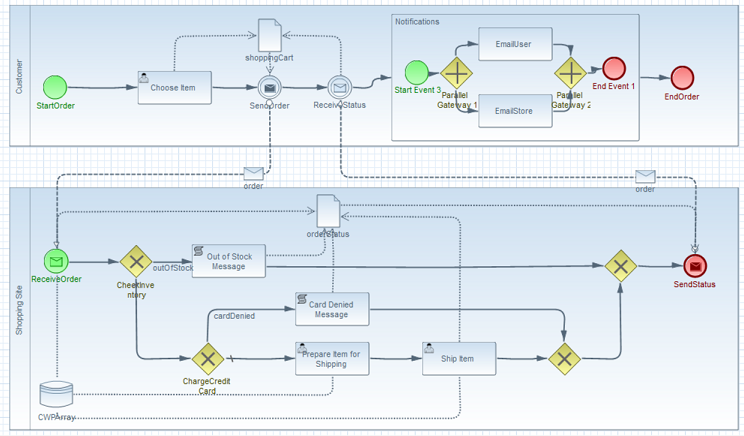
\includegraphics{shoppingFlow}
  \caption{A Shopping Cart Example}
  \label{fig:shoppingFlow}
\end{figure*}

\section{Background}\label{sec:background}
The translation is based on understanding of the BPMN language and the model checking language PROMELA.

\subsection{BPMN Structure and Semantics}

The model in Figure \ref{fig:shoppingFlow} represents a person checking out on an online store. This example represents all the features supported by this project in translation to PROMELA. A person chooses the item they want to buy and they submit and a send a request to the online store and wait for a response. The online store checks to see if the item is out of stock. If it is out of stock the item is not purchased. If the card was denied it does not purchase the item. Otherwise it prepares the item for shipment and begins shipment of item. Afterwards the Shopping Site sends the status back. When the customer receives the status back it starts a process to notify the customer and item owner. Then the process ends.

We first note that the example is split into two main logical pieces. These containers are called \emph{swim lanes} and each contain a start-event. Each swim lane represents a process that can run independently from each other. The swim lanes in our example are \emph{Customer} and \emph{Shopping Site}.

The tasks in the our example are of two varieties. There are abstract tasks like \emph{EmailUser} that are abstract and represent work only conceptually. There are also tasks like \emph{Out of Stock Message} that run code as part of their execution.

Sub-processes are similar to tasks. Instead of containing abstract work or code to run, they contain a process within them. The execution flow is the same as well. It gains a token, does its work (in this case a process) and passes the token on. In our example there is a \emph{Notifications} subprocess which notifies both users and owners of a store and does it all as single unit of work.

Gateways model decisions made in a BPMN process. Parallel gateways, as in the sub-process in \ref{fig:shoppingFlow}, are a way to choose multiple paths that run in parallel. Also in the diagram are \emph{exlusive} gateways as indicated by the X on the gateways. Consider the gateway \emph{CheckInventory}. Only one path in an exclusive gateway can be taken.  Either the different options are all equally likely and it randomly picks, or there are \emph{conditions} on the outward flows that decide what paths are possible. 
Gateways can diverge, as in the previous example, but they can also converge, back together. An exclusive gateway requires only one of the incoming flows to have a token in order to be enabled. This is the case for the two bottom right gateways in the diagram. 

BPMN uses \emph{Data stores}, represented with a cylinder, and \emph{Data Objects}, represented with a piece of paper,  to represent data. Data Objects are used to represent data that is local to a process and Data Stores are used to represent data that is global. This data can then be referenced using a data association line. 

The dark dashed lines with envelopes represent the way that BPMN uses messages to communicate between processes. In our example they are used to send an order to a website and receive a response back.

%seems a little unwieldy 
There is a special type of start-event that begins when it receives a message. There is a special type of end-event that sends a message before it ends its process.

There are also intermediate events which occur during the course of a process. Two such in our flow are the \emph{Message Throw} event \emph{SendOrder} and the \emph{Message Catch} event \emph{ReceiveStatus}. \emph{SendOrder} sends a message when it receives a token. \emph{ReceiveStatus} waits for a message before it finishes executing. 

%move to the translation section
% In the event that no flow default flow is defined and no options are executable it creates a run-time error.

\begin{figure*}
   \caption{PROMELA Example - Leader Election}
  \label{fig:promelaExample}

%include Promela code snippet to give examples
\begin{lstlisting}
#define N 3

chan channels[N] = [1] of {pid}

pid global_leader = 0;

proctype node(chan in, out) {
  pid leader
  out!_pid
endLO:
  do
  :: in?leader -> 
	 if
	 :: leader == _pid ->
		break
	 :: leader > _pid ->
		out!leader
	 :: else
	 fi
  od
  printf("leader = %d\n", leader)
  assert(leader == N)
  global_leader = N
}

init {
  byte index_in, index_out
  byte i
  atomic{
	for (i : 1 .. N) {
	  index_in = i - 1
	  index_out = i % N
	  run node(channels[index_in], channels[index_out])
	}
  }
endLO:
}
\end{lstlisting}
\end{figure*}
\subsection{PROMELA}

Consider the PROMELA example in Figure 
\ref{fig:promelaExample}. This PROMELA models Dijkstra's Leader Election Algorithm. A ring a of connected nodes are created. When a leader is chosen the choice is broadcast along the ring.

The first thing we notice is the term \emph{proctype}. It appears similar to a function, but the code within a proctype is run in its own processes and runs asynchronously from the other processes. In our example we also notice an init block. The init block is special type of process that starts when the PROMELA code begins to execute. 


An \emph{if-statement} in PROMELA differs in its definition in other languages. Lines 13 to 19 show an example of an if-statement. Each double colon represents an option that the if-statement may take. The choice of which option is executed is non-deterministic if multiple options are simultaneously true. If none of the options is true then the structure blocks and waits until one of the options becomes true.

A \emph{do-statement}  is similar to an if statement and an example can be seen from lines 11 to 20. A do-statement is essentially an infinite loop of an if-statement. A non-deterministic choice is made like an if statement and will block if no options are true. A do-statement must be exited explicitly as it is done on line 15 of the example.

Channels allow message passing in PROMELA. In our example the different processes representing nodes can communicate with their neighbors via channels. Message can be sent with a \emph{!-operator}  and received with a \emph{?-operator} . It is also possible to match on values in the channel when receiving.

There are couple of ways to validate properties in a PROMELA model. You can check safety properties by using \emph{assert} statements as at line 22 or write more complex properties using Linear Temporal Logic to check liveness requirements.
%not sure if I need this or not
%PROMELA's \emph{mtype} type is an enumerated type.

PROMELA does not support traditional functions. So to manage code re-usage we can use traditional C macros or SPIN provides \emph{inline} statements. Inline statements look like function calls with parameters. At execution the pseudo function call to a inline statement is replaced with the contents of the predefined inline statements and all the references to the parameters are replaced with what was passed in. Inline statements are used in our translation in Section \ref{sec:translation}.

\section{Translation}\label{sec:translation}

There are two major steps to the conversion of a BPMN diagram into PROMELA. The first is importing the BPMN structure. This step is not discussed in this paper and is assumed to have been done correctly. The next is creating the translation to PROMELA.

The main idea of the translation is represented with processes and a transition relationship represented with a PROMELA \emph{do-statement}. Movement within a process is created by having a \emph{guard} on every option of the do-statement. These guards usually are checking for one or two tokens that are coming in to an element within the BPMN flow. For instance in Figure \ref{fig:promelaSmall} on line 13 there is a guard that represents the sequence flow entering the \emph{token\_task1\_2} task. The do-statement will not execute the related code for the task until the counter that represents that incoming sequence flow has a value greater than zero. Once the guard becomes true and it enters the code associated with the element it will decrement the counter associated with the sequence flow.

%atomic
In order to cut down on the state space created we treat the code that executes after a guard in the do-statement atomically meaning that the schedule does not pre-empt the code in the block (although it may block of its own accord). When proctype processes are started in these blocks the run command is part of the atomic block but the process it starts is not. 


\subsection{Basic Helper Macros}
The following functions help to move tokens and check to see if transitions are enabled.

\begin{lstlisting}
inline has_token(token_count){
	(token_count > 0)
}
inline decrement_tokens(token_count){
	token_count--;
}
inline in_tokens(token_count) {
	(token_count > 0) -> token_count--;
}
inline double_in_tokens(token_count1,token_count2) {
	(token_count1 > 0 && token_count2 > 0) -> 
	token_count1--;
	token_count2--;
}
inline out_tokens(token_count) {
  token_count++;
}
\end{lstlisting}

\begin{itemize}
  \item \emph{has\_token} is used to check if there is a token in a sequence flow
  \item \emph{decrement\_tokens} is used to remove a token without moving it to another flow. 
  \item \emph{in\_tokens} is used in general to represent the condition sequence flow having a token and the token being consumed by a BPMN element and so the token counter is decreased. 
  \item \emph{double\_in\_tokens} is similar but requires two flows each with a token and the decrements both flows as appropriate. It is important to note that in this translation, objects requiring more than two flows to activate must use gateways to collect up flows by pairs (see Section \ref{sec:gateways}). 
  \item \emph{out\_tokens} encapsulates the idea of a BPMN element finishing its execution and putting a token onto an outbound sequence flow.
\end{itemize}

Also in the helper functions there are parameters starting with \emph{messageNumber}. They are used for debugging statements. This is because PROMELA cannot pass string literals. So we replace the string literals with constant integers that can be post-processed into sensible message. More info is given in Section \ref{sec:runningTranslation}.

\subsection{Processes}
BPMN Processes are represented in PROMELA as proctypes. Every process is given as a parameter a report channel. This channel is used to report how a process terminated (i.e., normally, abnormally, threw an error). It is also used, in the case of a sub-process, to return control to the parent process.

In every process there is also a check to see if the process is ending abnormally. The BPMN specification defines ending abnormally as follows:
\begin{quote}
For a Process instance to become completed, all tokens in that instance MUST reach an end node, i.e., a node without
outgoing Sequence Flows. A token reaching an End Event triggers the behavior associated with the Event type, e.g.,
the associated Message is sent for a Message End Event, the associated Signal is sent for a Signal End Event, and
so on. If a token reaches a Terminate end-event, the entire Process is abnormally terminated \cite{BPMNSpecification}.
\end{quote}

At the end of the process all sequence flow counters are checked for values. If any have a value greater than zero then the process is abnormally terminated and it sends an abnormal type back on the report channel. If it does end with anything other than normal, it prints out all of the sequence flow counters.

\subsection{Sub-processes}

Sub-processes inherit all of the same translation techniques as normal processes. They are implemented with two guards in the do-statement (Figure \ref{fig:subprocessSnippet}). One of the transitions starts the sub-process with a \emph{run} command and gives a channel local to the process as the report channel (line 4). The other guard (line 6) waits to receive on the channel and when it receives a message it first checks for a normal termination to the sub-process, if it is not normal it reports it. Then it puts a token on the outgoing flow.

\begin{figure}
\begin{lstlisting}
:: ...
::in\_tokens(token\_5\_10) -> 
	atomic{
	run subprocess(cwpArrayIndex, subprocess_channel); 
	}
::len(subprocess\_channel) > 0 ->
	atomic{
	mtype tempS;
	subprocess_channel?tempS;
	if
		::tempS==normal;
		::else -> reportChannel!tempS;
	fi
	out_tokens(token_6_11)
	}	
:: ...
\end{lstlisting}

\caption{Subprocess Snippet}
 \label{fig:subprocessSnippet}
\end{figure}


\subsection{Data}\label{sec:data}

Data Objects and Data Stores represent data in BPMN. These two objects are given a data type and a capacity representing how many objects they can hold (We have extended Data Objects to have capacity). With this information we can declare them as respectively local and global variables respectively (i.e., a data-store is global and a data-object is local). The name of the variable produced is the same as the name of the Data Object or Data Store. These variables will be available for use in script tasks and gateway conditions.

Data Types can be primitive types or specified in manner similar to C structs. Structures are defined with the keyword \emph{typedef} in PROMELA. Basic types can optionally provide a maximum value and/or a default value. If no maximum value is specified then it is set to 256.  PROMELA already automatically defaults all primitive types to zero. Future work to automate the conversion from BPMN XML files to the data-structure for the translation will use XSD files to define the type of the data-objects and data-stores in the BPMN model. These type of details are normal and expected for any BPMN execution environment that does more than random simulation along flows.

All basic type fields defined (on their own or in a stucture)  generate \emph{\#define} statements in PROMELA that define how large of value is permitted for every variable. The translation expects a basic integer input for all integer values. However, internally the most restricted data type possible is used depending on the maximum value defined. If it is less than 2 we use a bit, less than 256 we use a byte, less than 32,768 a short and otherwise we use an int. Currently negative numbers are not supported.



\subsection{Tasks}

Script Tasks allow you to manipulate data with PROMELA code that is executed as part of the script task. The PROMELA code is added to a field that is part of the BPMN specification. It simply inserts the code specified directly into the PROMELA translation. It may use constants defined for maximum values and variables defined to represent Data Stores and Data Objects. 

Some tasks in BPMN, like manual tasks, are meant to represent work done by a person. This may need to be represented by code. In order to facilitate this functionality we abuse the \emph{Documentation} for the manual task element field occasionally to use arbitrary PROMELA code and essentially convert a manual task into a script task.

There is also a variable that is always available that indicates which instance of the BPMN diagram is currently being used called \emph{token id}. The name of this variable is the name of Data Store concatenated with \emph{Index}. If there is no Data Store then it uses the name \emph{token\_id}. 

In the case of our Shopping Cart example this is extremely important. Imagine that two BPMN instances are started to represent two different Customers. They both send their orders to the Shopping Site. However, when the Shopping Site sends a message back which Customer should receive the message? Intuitively we understand that it should be the same customer that initially sends the order. The \emph{token id} can be used as a key to resolve that issue.



\subsection{Events and Messages}

As mentioned previously start-events have no inbound sequence flows. For the purposes of our translation we give all start-events an implicit inbound sequence flow and set the counter for it to one to begin the process.

End-events have no outgoing sequence flows. So at the end of the execution of a end-event it uses a \emph{break} statement to exit the transition loop.

Several of the events that are covered deal with handling message passing. Figure \ref{fig:messageTranslation} shows the translation of these events.

Message end-events begin and end like a normal end-event. They send a message over a channel to be picked up by a message catch event. Line 20 shows the pivotal part of an end event where it sends a message with the \emph{token id} and the message payload. 

Message Throw events are similar to message end-events conceptually, but happen in the middle of a process. Line 5 shows a Message throw event using a \emph{run} command to start a new process and pass in the message into the parameters of the new process without using a channel. Currently the translation assumes a that message send throw events go directly to a start-event. 

Message Catch events do not execute until they are both enabled and have a message ready to receive. Once those requirements are met, the payload of the channel is unloaded into the variable representing the Data Object it is connected to. The guard looks like line 9 where there must be a token and it checks to see if there is a message on the channel it can receive. The messages are matched on the \emph{token id} (\emph{cwpArrayIndex}) to make sure that the receiver is a process started by the same BPMN instance.

Message start-events are essentially equivalent to a normal start event once the process begins. The defining difference is that a process that begins with a message start event is not automatically started when the program begins, but must be started with a Message Throw event.

\begin{figure}
\begin{lstlisting}
::...
/*Message Throw*/
::in_tokens(token_3_8) -> 
	atomic{
	run process_ShoppingSite(cwpArrayIndex, reportChannel, shoppingCart)
	out_tokens(token_4_9)
	}
/*Message Catch*/
::token_4_9 > 0 && chan_MessageFlow2??[eval(cwpArrayIndex), shoppingCart]->
	atomic{
	chan_MessageFlow2??eval(cwpArrayIndex), shoppingCart;
	decrement_tokens(token_4_9);
	print(997/*ReceiveStatus-4*/);
	out_tokens(token_5_10)
	}
/*Message End Event*/
::in_tokens(token_SendStatus_19) -> 
	atomic{
	print(982/*SendStatus*/);
	chan_MessageFlow2!cwpArrayIndex, orderStatus;
	break;
	}
:: ...
\end{lstlisting}

\caption{Message Events Translation}
 \label{fig:messageTranslation}
\end{figure}



\subsection{Gateways}\label{sec:gateways}

We make the assumption that gateways can only diverge to and converge from a maximum of two flows. Then multiple gateways can be chained together to accomplish any desired gateway configuration. The gateways we translate using helper functions (Figure \ref{fig:exclusiveGatewayFunctions} and Figure \ref{fig:parallelGatewayFunctions}). All of the parameters in the helper functions that begin with \emph{inseq} refer to inbound sequence flows and parameters that begin with \emph{outseq} refer to outbound sequence flows.

For exclusive gateways we define three different helper functions: \emph{xor\_join}, \emph{xor\_fork\_default}, and \emph{xor\_fork}   (Figure \ref{fig:exclusiveGatewayFunctions} ). The first is for when flows converge and the other two are for when they diverge. 

Diverging exclusive gateways can have expressions on outbound flows that indicate whether or not the sequence flow can be used. There is also the notion of a default flow that is true if the other flow is not. If one of the flows is a default flow \emph{xor\_fork\_default} is used otherwise \emph{xor\_fork} is used. The parameters between these two functions vary slightly because a default flow does not need a condition. If there is no default flow and no flow is true then we get a run-time error. This error is handled on line 24 by using the \emph{reportChannel} to report an error back to the parent process.


\begin{figure}
\begin{lstlisting}
inline xor_join(messageNumber, inseq,inseq2, outseq){
	((inseq > 0) || (inseq2 > 0) ) ->
	atomic {
	print(messageNumber)
	if 
	:: in_tokens(inseq) -> out_tokens(outseq)
	:: in_tokens(inseq2) -> out_tokens(outseq)
	fi
	}
}

inline xor_fork(inseq,messageNumber1,expr1, outseq1, messageNumber2, expr2,outseq2,reportChannel){
  in_tokens(inseq) ->
  atomic {
	if
	::(expr1) ->
	   print(messageNumber1)
	   out_tokens(outseq1)
	::(expr2) ->
	   print(messageNumber2)
	   out_tokens(outseq2)
	:: else ->
	   printf("xorsplit exception");
	   reportChannel!xor_split_false;
	   break;
	fi
  }
}

inline xor_fork_default(inseq,messageNumber1,expr1, outseq1, messageNumber2,defaultSeq){
  in_tokens(inseq) ->
  atomic {
	if
	::(expr1) ->
	   print(messageNumber1)
	   out_tokens(outseq1)
	:: else ->
	   print(messageNumber2)
	   out_tokens(defaultSeq)
	fi
  }
}
\end{lstlisting}

\caption{Exclusive Gateway Functions}
 \label{fig:exclusiveGatewayFunctions}
\end{figure}


For parallel gateways (Figure \ref{fig:parallelGatewayFunctions}) we define two different helper functions. One for when the flows diverge and one for when they converge. There are no expression on the flows. \emph{parallel\_fork} puts a token on both outgoing sequence flows. \emph{parallel\_join} requires that both incoming sequence flows have tokens before the gateway is enabled.


\begin{figure}
\begin{lstlisting}
inline parallel_fork(inseq,messageNumber, outseq1,outseq2){
  in_tokens(inseq) ->
 
  atomic {
   print(messageNumber)
	out_tokens(outseq1)
	out_tokens(outseq2)
  }
}

inline parallel_join(messageNumber, inseq1,inseq2,outseq){
  	double_in_tokens(inseq1,inseq2)-> 
	atomic {
	print(messageNumber)
 	out_tokens(outseq)
	}
}
\end{lstlisting}

\caption{Parallel Gateway Functions}
\label{fig:parallelGatewayFunctions}
\end{figure}
\subsection{Running the Translator}\label{sec:runningTranslation}

%instantiating BPMN
We \emph{instantiate} a BPMN model N number of times where N is the capacity of the Data Store and with the lack of a Data Store it is a parameter given to the translator. Each instantiation has a unique \emph{token id}. For each \emph{instantiation} of the model we start a process for every swim lane that begins with a normal start-event. Each process start is given as parameter, the \emph{token id}, that refers to the instantiation of the BPMN diagram.

%simulation mode
In simulation mode and error traces it is helpful to have print statements denoting what happened. While it is possible to print string literals in PROMELA, it is not possible to pass string literals in the code which makes it hard to use inline statement templates. Our solution to this is to print message numbers that are translated into text via an awk-script. This script is generated along with the PROMELA file and using a standard pipe we can transform the output of traces and simulations. In the code itself the string literal is denoted in a comment. Figure \ref{fig:awkExample} has an example of what the output of simulation would look with and without an awk-script. Line 2 starts the original output that just has numbers. Line 8 starts the output with the awk-script translating the numbers into useful output.


\begin{figure}
\begin{lstlisting}
spin generatedPromela.pml
          message: 1000
          message: 999
          message: 998
              message: 983
...
spin generatedPromela.pml | awk -f awk.txt
          ReceiveStatus
          SendOrder
          StartOrder
              join1: xor join
...
\end{lstlisting}
\caption{awk-script example}
\label{fig:awkExample}
\end{figure}		  


%Talk about assertion of normal termination.

%Talk about associating a Data Object with a message type event

\section{Validation}

We manually wired up our Shopping Cart example (see Figure \ref{fig:shoppingFlow}). With that we were able to generate working PROMELA code. The model varied in the number of states that it generated depending on the sizes of the variables specified by the users. 
Our main experiment was performed on the \emph{Shopping Cart} flow. The flow encapsulates the majority of the BPMN that we are implementing as a part of this conversion.

Running one instance of the Shopping Cart example (with the maximum value of every variable being zero) gave us 231 states (Figure \ref{fig:spinResults}). We were able to have up to three instances with 49,568,763 states and no invalid end states. There is an assert in the code that verifies that all processes are terminated normally. This BPMN model had no invalid terminations. Verifying 4 concurrent instances, meaning 4 unique customers shopping at the same time, did not complete within an hour

The results given by SPIN indicated for our test flow indicated that all of the processes ended correctly. This is seen by the lack of an assertion fail and how to the output shows that certain places were unreachable in the code. The code that is unreachable is error handling code.

Our experiments showed that the state space can easily become unmanageable. For example, in our test flow there was code in a script-task to non-deterministically set the value for several variables. The state space size depended greatly upon the range of valid valid values given for the variables. With one instance and increasing the maximum value of the variables from 0 to 255 the number of states increased from 231 states to 56,841 states. 

In order to handle larger BPMN Models or more instances abstraction techniques will need to be employed.

\section{Related Work}

There has not been much work done in this field to the author's knowledge. Choreographies, a special branch of BPMN diagrams that focus on communication between multiple processes has been explored in \cite{choreography}. It does not allow conversion of work-flow processes. 

Other work has been done converting BPEL, another work-flow language, to PROMELA. There has also been work to convert BPMN to BPEL \cite{bpelToPromela}. So there is a theoretical path to convert BPMN to PROMELA through the intermediate step of BPEL. The work in BPEL however is focused on modeling web service calls, so the effectiveness of the translation is not clear. It is also not clear that using a two step translation would allow for enough control to manage state space explosion.  

There are other examples of BPMN to Petri Nets and other Petri Net to PROMELA conversions \cite{petrinetToPromela}. Petri nets are mathematically well defined and that formalism lends itself well to verifying systems. That formalism in transitions with Petri nets inspired our own solution \cite{petrinetInspiration}. However, they do not take into consideration data manipulation which we feel is important to model as much as the transitions themselves. More critically, without data as a first class citizen in the model (which is not the case with most Petri Net formalisms), it is very difficult to verify if a BPMN process accomplishes its intended work. In other words, does the process transform its input into the intended output in a valid way. 

While there are translations from BPMN to PROMELA we feel that none have been able to translate work-flow processes while handling data correctly. To our knowledge this work is unique in its translation techniques.

\section{Conclusions and future work.}

This paper presented a translation from BPMN to PROMELA that accurately represents the original BPMN model. The translation was shown to cover only a subset of BPMN functionality, but still has enough support to represent real world processes. The translation uses a novel approach that represents transitions in BPMN models within do-statements in PROMELA proctypes. Other details of the translation are laid out with helper functions and clear translation techniques. Initial results indicate that the translation is accurately representing the BPMN models.


Here are some things we would like to do in the future:
\begin{itemize}
  \item Implement BPMN Elements not included in our translation such as the \emph{Inclusive Gateway} and back-edges. The gateway will require flow-analysis to determine which edges merge and the loop will require some way to track iteration counts on tokens that flow around the loop. Neither of these concepts are well (if at all defined) in the BPMN standard surprisingly.
  \item Explore folding all swim lane process for a single BPMN instance into a single process. This complicates the namespace and scope of variables. Then a comparison of state space could be made with the current translation techniques.
  \item Apply abstraction techniques to deal with state space explosion.
  \item Write a preprocess to take the loose syntax that BPMN allows and translate into a stricter form. For example, allow a gateway to have more than two incoming sequence flows and split it into multiple chained gateways that each only have two incoming sequence flows.
  \item Make it easier for non-expert users to use. 
\end{itemize}

\section{Assumptions and Notes}
\begin{itemize}
  \item Mtypes are defined on a global basis. This means that different mtype variables can share mtype values; it also means that any mtype variable can receive any mtype value even if it is not related in the set defined by the user. We leave it to the user to correctly assign values.
  \item Every process, including sub-processes, has a single start-event and end-event.
  \item There can only be one Data Store.
  %deviations
 \item We add the ability for a data object to have a capacity like a Data Store can.
  %conventions
  \item Data Objects and Data Stores have names that have no spaces and are compatible as a variable name in PROMELA.
  \item No element has more than two sequence flows that enter and more than two that leave. Those that have two entering must only have one that leaves and vice versa. Gateways are chained together to get the functionality of more than one choice. We also add the constraint the all BPMN diagrams must have explicit start and events for every process. 
  \item The scope of data in our system differs from the BPMN specification for Data Objects. In the specification the scope of a Data Object is for the current process and all sub-process. In our implementation the scope of a Data Object is only for the current process and not sub-processes.The scope of data in our system differs from the BPMN specification for Data Objects. In the specification the scope of a Data Object is for the current process and all sub-process. In our implementation the scope of a Data Object is only for the current process and not sub-processes.
  
  \item There can be at most 1000 print messages.
  
  \item As of yet we have not designed the system to work with back edges in the BPMN models. The syntax of BPMN is not clear on what is acceptable behavior. 

  \item We do not have inclusive gateways. They are complicated because you do not know until run time which paths will be taken. In the case of an exclusive gateway that is acceptable, but with an inclusive gateway it acts similar to a parallel gateway join. So for every outgoing flow of an inclusive gateway that is activated it must wait for all of those to join together later. It is something that may be implemented eventually.
  
  \item Messages cannot send Typedefs that have arrays in them because of a limitation in PROMELA.
  
\end{itemize}

\begin{figure*}
   \caption{SPIN Results}
  \label{fig:spinResults}


\begin{lstlisting}
(Spin Version 6.4.6 -- 2 December 2016)
	+ Partial Order Reduction

Full statespace search for:
	never claim         	- (none specified)
	assertion violations	+
	cycle checks       	- (disabled by -DSAFETY)
	invalid end states	+

State-vector 36 byte, depth reached 27, errors: 0
       22 states, stored
        1 states, matched
       23 transitions (= stored+matched)
       13 atomic steps
hash conflicts:         0 (resolved)

Stats on memory usage (in Megabytes):
    0.001	equivalent memory usage for states (stored*(State-vector + overhead))
    0.280	actual memory usage for states
  128.000	memory used for hash table (-w24)
    0.534	memory used for DFS stack (-m10000)
  128.730	total actual memory usage


unreached in proctype process_SimpleFlow
	generatedPromela.pml:37, state 59, "printf('token_conParGW_4 %d\n',token_conParGW_4)"
	generatedPromela.pml:39, state 61, "printf('token_divParGW_1 %d\n',token_divParGW_1)"
	generatedPromela.pml:40, state 62, "printf('token_end_6 %d\n',token_end_6)"
	generatedPromela.pml:41, state 63, "printf('token_task1_2 %d\n',token_task1_2)"
	generatedPromela.pml:42, state 64, "printf('token_task2_3 %d\n',token_task2_3)"
	generatedPromela.pml:43, state 65, "reportChannel!abnormal"
	(6 of 69 states)
unreached in init
	(0 of 12 states)

pan: elapsed time 0 seconds

\end{lstlisting}
\end{figure*}

\bibliographystyle{plain}
\bibliography{bibliography.bib}

%\end{multicols}
\end{document}
